% Self-contained IEEE manuscript. Compile twice with pdfLaTeX.
\documentclass[journal]{IEEEtran}
\usepackage[T1]{fontenc}
\usepackage[utf8]{inputenc}
\usepackage{newtxtext,newtxmath}
\usepackage{microtype}
\usepackage{graphicx}
\usepackage{booktabs,tabularx,array}
\usepackage{hyperref}
\usepackage{cite}
\usepackage{tikz}
\usetikzlibrary{arrows.meta,positioning}
\usepackage{pgfplots}
\pgfplotsset{compat=1.18}
\hypersetup{hidelinks}
\title{ARIA: An Auditable Offline Reinforcement-Learning Architecture for Adaptive Mock Interviews}
\author{Raghav Samir Sejpal and Krissh Verma%
\thanks{R. S. Sejpal and K. Verma are with the School of Computer Science and Engineering, Vellore Institute of Technology, Vellore, Tamil Nadu, India (e-mail: raghavsamir.sejpal2023@vitstudent.ac.in; krissh.verma2023@vitstudent.ac.in). This work was supervised by Dhivyaa C. R.}}
\begin{document}
\maketitle

\begin{abstract}

Adaptive mock-interview systems must do more than generate plausible questions: they must maintain an interpretable estimate of candidate evidence, select actions without extrapolating beyond observed behavior, and state which claims their evaluation can support. This paper presents ARIA, an Autonomous Reinforcement-Based Interview Agent whose offline architecture combines calibrated belief estimation with Implicit Q-Learning (IQL). The evaluated state contains 33 features and supports eight interview actions. A synthetic corpus contains 600 episodes and 9,018 transitions, partitioned through 33 identity components into 422 training, 87 validation, and 91 locked-test episodes. On the locked synthetic test, the calibrated belief model achieved 0.9121 accuracy, 0.9168 macro-F1, 0.9227 balanced accuracy, 0.0870 expected calibration error, and 0.1395 Brier score. A paired comparison with the preceding calibration model improved accuracy by 0.1209 and macro-F1 by 0.1158; identity-component bootstrap intervals were positive for both measures. These are belief-estimation results, not learned-policy outcomes. A separate clipped weighted-importance-sampling diagnostic on 1,405 validation transitions estimated reward 0.4618 with an effective sample size of 1003.5, but it does not satisfy the policy-release criterion. The current live application assigns fixed evidence values and cycles through three actions; it does not execute the learned IQL policy. In light of 2026 work on multimodal mock interviews, trait-activated interview data, psychometric fairness, and disability exclusion, ARIA is positioned as an experimental system rather than a validated hiring instrument. Human construct validity, accessibility, subgroup fairness, live integration, and fresh learned-policy rollouts remain required.


\end{abstract}
\begin{IEEEkeywords}
adaptive interviewing, automated video interview, calibration, Implicit Q-Learning, multimodal assessment, offline reinforcement learning, auditability, synthetic data
\end{IEEEkeywords}
\section{Introduction}

Automated interviews increasingly combine language, speech, and visual behavior. Earlier work showed that multimodal cues can predict interviewer ratings \cite{hemamou2019hirenet}--\cite{naim2018automated}, \cite{hemamou2023multimodal}, \cite{nguyen2014hireme}, \cite{chen2016monologue}, \cite{lv2024window}, \cite{suen2020agent}, \cite{chen2016doc2vec}. Psychometric studies subsequently asked harder questions about reliability, generalizability, ground-truth quality, and whether model scores correspond to intended constructs \cite{hickman2022personality}, \cite{liff2024psychometric}, \cite{hickman2025smart}, \cite{koutsoumpis2024psychometric}, \cite{hickman2024training}, \cite{hickman2021language}, \cite{zhang2025personality}. This progression matters: a predictive model can reproduce a rating without establishing that the rating is job-relevant, stable, fair, or useful for deciding what to ask next.


Adaptation introduces a sequential decision problem. The interviewer observes incomplete evidence, updates a belief over skills, and chooses a next action. Computerized adaptive testing provides a precedent for uncertainty-aware item selection \cite{li2026deepcat}, while offline reinforcement learning provides tools for learning from logged trajectories when online exploration would be inappropriate \cite{kostrikov2021iql}, \cite{thomas2015hcope}--\cite{patterson2023empirical}. Yet neither adaptation nor offline learning automatically establishes beneficial policy behavior. Evaluation must separate state estimation from action selection and must make behavior-policy mismatch visible.


The governance burden is especially high in hiring. Research has documented unsupported vendor claims, instability, demographic disparities, disability exclusion, contested emotion inference, and opacity in audit regimes \cite{raghavan2020bias}, \cite{tippins2021concerns}, \cite{rhea2022stability}--\cite{fabris2025survey}, \cite{luria2026disability}--\cite{wilson2021fairalgorithms}, \cite{hunkenschroer2022ethics}--\cite{aizenberg2023autonomy}, \cite{ingber2025emotion}, \cite{roemmich2023values}, \cite{kassir2022context}, \cite{li2021practice}--\cite{gerchick2025audits}, \cite{fisher2024disability}, \cite{yam2021impact}--\cite{roemmich2023privacy}, \cite{raji2022oversight}. These concerns are not peripheral ethical add-ons. They affect the validity of observations, the accessibility of the procedure, and the meaning of any score.


Recent 2026 literature sharpens the problem. PolyInterview demonstrates role-conditioned planning, answer-aware follow-ups, and multimodal feedback at platform scale, while also reporting weaker faithfulness when generating polished responses \cite{wen2026polyinterview}. Two CHI studies show that digitized assessments and AI interviews can impose access labor, normative behavioral expectations, information asymmetry, and privacy burdens on disabled applicants \cite{luria2026disability}, \cite{kameswaran2026surveilling}. A psychometric synthesis maps machine learning fairness criteria to long-standing testing concepts and emphasizes bias propagation through sequential assessment decisions \cite{cheng2026fairness}. A systematized review describes a shift from matching models toward recruiting agents \cite{zhao2026recruitingagents}, and a CSCW study finds that applicants increasingly expect interactive, controllable AI interview experiences \cite{sakib2026expecting}. AVI-Personality supplies trait-activated prompts, expert behaviorally anchored ratings, and a large multimodal dataset, but its multimodal gains over strong text baselines are modest \cite{zhang2026avipersonality}. Accordingly, ARIA cannot claim novelty merely from combining multimodality, generated questions, or adaptive interaction.


This study asks three questions. First, what state, action, belief, data, and policy contracts define the evaluated ARIA system? Second, what does the locked synthetic evaluation establish about belief estimation and offline policy diagnostics? Third, which claims remain unsupported because learned-policy rollouts, live integration, and human validation are incomplete?


The contribution is fourfold. First, we define a 33-dimensional belief-aware interview state and an eight-action policy interface. Second, we evaluate an identity-isolated synthetic trajectory corpus and a locked belief test with calibration and class-sensitive metrics. Third, we report IQL training and a diagnostic off-policy estimate while preserving the distinction between value estimation and policy effectiveness. Fourth, we expose the boundary between the evaluated offline pipeline, the simplified live application, and the studies still required for validity, fairness, accessibility, and deployment. This scope follows the engineering-forward presentation common in relevant IEEE Access work \cite{kim2023fairness}, \cite{putra2024magbert}, \cite{suen2019personality}, while narrowing claims to the completed experiments.


\section{Related Work}

\subsection{Structured and Automated Interviews}

Structured interviews have stronger foundations than unstructured impressions, but validity depends on question design, scoring, and criterion evidence \cite{levashina2014structured}, \cite{mcdaniel1994validity}. Computational interview research initially inferred hirability or performance from verbal and nonverbal behavior \cite{naim2018automated}, \cite{nguyen2014hireme}, \cite{chen2016monologue}, \cite{chen2016doc2vec}. HireNet and later hierarchical attention models represented frames, words, answers, and interviews at multiple levels \cite{hemamou2019hirenet}, \cite{hemamou2023multimodal}. Other systems predicted communication skill or personality from asynchronous video \cite{suen2020agent}, \cite{suen2019personality}. These studies established technical feasibility, not interchangeability between behavioral cues and occupational competence.


Recent psychometric work makes that distinction explicit. Automated personality and competency scores require reliability, convergent or criterion validity, and generalizability checks \cite{hickman2022personality}, \cite{liff2024psychometric}. Performance depends on training-sample size, label reliability, and language model choice \cite{hickman2024training}, while automated speech recognition error can propagate into interview scores \cite{hickman2025asr}. Koutsoumpis et al. examine personality and interview performance jointly \cite{koutsoumpis2024psychometric}, and Hickman et al. test cognitive ability scoring, behavioral modes, and bias \cite{hickman2025smart}. Faking, impression management, and candidates' use of AI further complicate score interpretation \cite{hickman2025faking}. ARIA therefore treats its low/medium/high labels as synthetic engineering targets, not validated occupational constructs.


\subsection{Multimodal Fusion and IEEE Access Comparators}

Multimodal systems combine lexical, acoustic, and visual streams, but more modalities do not guarantee better measurement. Booth et al. found that verbal features were competitive with a combined model and that visual information could worsen fairness indicators \cite{booth2021bias}. Window-consistency fusion \cite{lv2024window}, Doc2Vec fusion \cite{chen2016doc2vec}, and multimodal attention \cite{hemamou2023multimodal} offer increasingly elaborate representations, while uncertainty-aware spoken-language assessment shows why predictive confidence should be modeled rather than ignored \cite{malinin2017uncertainty}.


Three IEEE Access papers are direct structural and technical comparators. Suen et al. presented an end-to-end TensorFlow personality-recognition pipeline from asynchronous video \cite{suen2019personality}. Kim et al. introduced fairness-aware multimodal learning using distributional regularization and continuous-score fairness measures \cite{kim2023fairness}. Putra et al. proposed MAG-BERT-ARL, reporting performance and fairness trade-offs without requiring sensitive attributes at inference \cite{putra2024magbert}. Together, these papers motivate ARIA's modular description, explicit metrics, and comparative tables. They also caution against a single aggregate accuracy claim: Kim et al. require group labels during training, whereas Putra et al. avoid them but report inconsistent behavior across fairness criteria \cite{kim2023fairness}, \cite{putra2024magbert}. ARIA has not yet conducted either form of subgroup evaluation.


The 2026 AVI-Personality dataset further shows that targeted questions designed under Trait Activation Theory can strengthen self--other agreement and that trained raters using behaviorally anchored scales provide a more defensible label source than crowd impressions \cite{zhang2026avipersonality}. Its strongest multimodal benchmark only modestly exceeds strong text baselines. This supports a modality-ablation requirement for ARIA rather than an assumption that webcam and prosody features add valid information.


\subsection{Adaptive Questioning, Item Generation, and Offline RL}

Question adaptation has roots in computerized adaptive testing. Deep CAT combines multidimensional latent-state estimation with non-myopic selection \cite{li2026deepcat}. Skill-oriented generation and recommendation can connect job descriptions to interview questions \cite{qin2023question}, while generative-AI item-development studies demonstrate the need for human review of generated items \cite{segall2025items}. PolyInterview adds role-conditioned plans and answer-aware probing \cite{wen2026polyinterview}. These approaches make broad novelty claims about adaptive questioning untenable; ARIA's distinction is an inspectable state-action contract around a conservative offline learner.


IQL learns value by expectile regression and extracts a policy through advantage-weighted behavioral cloning, reducing explicit evaluation of unsupported actions \cite{kostrikov2021iql}. Nonetheless, offline RL remains vulnerable to distribution shift and optimistic evaluation. High-confidence OPE separates point estimates from reliable bounds \cite{thomas2015hcope}; empirical OPE comparisons show sensitivity to horizon, mismatch, and model error \cite{voloshin2019ope}; and empirical RL guidance emphasizes protocols, seeds, uncertainty, and held-out evaluation \cite{patterson2023empirical}. ARIA consequently uses weighted importance sampling only as a diagnostic and requires fresh rollouts before claiming policy improvement.


\subsection{Fairness, Accessibility, Privacy, and Applicant Experience}

Algorithmic-hiring reviews identify recurring gaps between vendor claims, validation practice, and governance \cite{raghavan2020bias}, \cite{tippins2021concerns}, \cite{fabris2025survey}, \cite{hunkenschroer2022ethics}, \cite{kassir2022context}, \cite{hughes2025inequalities}, \cite{zhao2026recruitingagents}. External stability audits reveal sensitivity to irrelevant resume changes \cite{rhea2022stability}. Audit frameworks and field studies show that access, documentation, independence, and institutional incentives constrain what audits can establish \cite{kazim2021audit}, \cite{wilson2021fairalgorithms}, \cite{mihaljevic2023auditing}, \cite{gerchick2025audits}, \cite{costanzachock2022auditors}, \cite{raji2022oversight}. The literature therefore supports system-level evidence ledgers, not one-time parity reports.


Applicant reactions are equally consequential. Algorithmic evaluation can reduce perceived justice and acceptance, particularly in high-stakes settings \cite{acikgoz2020justice}, \cite{oostrom2023reactions}, \cite{pyle2024justice}, \cite{langer2019acceptance}, \cite{liu2023uncertainty}, \cite{hilliard2022perceived}. Emotion-AI studies raise concerns about autonomy, emotional labor, identity, workplace surveillance, and privacy \cite{ingber2025emotion}, \cite{roemmich2023values}, \cite{roemmich2023privacy}. Recruiter studies show that operational practice may depart from formal model descriptions \cite{li2021practice}. Human-rights and contextual accounts argue for impact assessment and contestability rather than a purely technical definition of fairness \cite{sanchezmonedero2020discrimination}, \cite{hunkenschroer2022ethics}, \cite{sloane2022auditability}, \cite{aizenberg2023autonomy}, \cite{kassir2022context}, \cite{yam2021impact}.


Disability scholarship shows why aggregate demographic metrics are insufficient. Technical and legal analyses identify accommodation and proxy-discrimination risks \cite{buyl2022disability}, \cite{tilmes2022disability}, \cite{fisher2024disability}. Modified question wording can affect autistic and neurotypical responses differently \cite{benson2024autistic}. In 2026, Luria et al. found that 9 of 17 disabled participants could not complete at least one simulated digitized assessment, while Kameswaran et al. documented normative scoring expectations, loss of interview mutuality, and privacy concerns across 19 disabled job seekers \cite{luria2026disability}, \cite{kameswaran2026surveilling}. These studies motivate accessible alternatives, candidate control, human review, and an explicit prohibition on using ARIA as an autonomous screening tool.


\subsection{Research Gap}

The literature contains strong work on structured interviewing, multimodal scoring, adaptive item selection, offline RL, and algorithmic-hiring governance. What remains comparatively underdeveloped is a system-level account that connects: (i) an explicit interview belief state; (ii) identity-safe trajectory construction; (iii) calibrated belief evaluation; (iv) a conservative offline policy; (v) OPE limitations; and (vi) the live execution path. Recruiting-agent reviews call for more integrated evaluation and governance \cite{zhao2026recruitingagents}, and 2026 user studies demand interactivity without sacrificing agency or access \cite{luria2026disability}, \cite{kameswaran2026surveilling}, \cite{sakib2026expecting}. ARIA addresses the narrower engineering gap of traceable evaluation separation, not the broader scientific gap of real-world interview validity. Table~\ref{tab:related-comparison} positions this scope against the closest 2026 studies.


\begin{table*}[t]
\caption{Comparison With Recent Interview and Assessment Research}
\label{tab:related-comparison}
\centering
\small
\begin{tabularx}{\textwidth}{>{\raggedright\arraybackslash}X>{\raggedright\arraybackslash}X>{\raggedright\arraybackslash}X>{\raggedright\arraybackslash}X>{\raggedright\arraybackslash}X}
\toprule
Work & Data and modality & Adaptation & Evaluation emphasis & Boundary relevant to ARIA \\ \midrule
PolyInterview (2026) \cite{wen2026polyinterview} & 1,564 sessions; text, audio, video & Answer-aware follow-ups & Expert quality ratings & No criterion-validity or employment-outcome evidence \\
Luria et al. (2026) \cite{luria2026disability} & 17 disabled participants; simulated assessments & None & Qualitative access and exclusion & Assessment completion can itself be inequitable \\
Kameswaran et al. (2026) \cite{kameswaran2026surveilling} & 19 disabled job seekers & User-requested responsiveness & Qualitative surveillance and autonomy & AI interviews can remove mutuality and disclosure control \\
Cheng (2026) \cite{cheng2026fairness} & Conceptual psychometric/ML synthesis & Sequential testing workflow & Fairness definitions and bias propagation & Fairness must be tested across the full pipeline \\
AVI-Personality (2026) \cite{zhang2026avipersonality} & 646 participants; 3,876 videos & Trait-activated prompts & Reliability, validity, fairness, MSE & Grounded labels and modality ablations are essential \\
ARIA (this work) & 600 synthetic episodes; 9,018 transitions & Offline IQL over eight actions & Calibration, lineage, diagnostic OPE & No human validity or policy-effectiveness claim \\
\bottomrule
\end{tabularx}
\end{table*}

\section{Problem Formulation}

\subsection{System Objective}

ARIA treats adaptive interviewing as a partially observed sequential decision problem. At turn $t$, the system receives response evidence $o_t$, maintains a belief $b_t$ over skill level, and selects an interview action $a_t$ from a set of eight valid actions. The immediate engineering objective is to estimate the belief reliably and learn a conservative action policy from logged synthetic trajectories. The present evaluation separates belief-estimation accuracy from policy value so that classification performance is not interpreted as evidence that adaptive questioning improves an interview.


For a trajectory $\tau=(s_0,a_0,r_0,\ldots,s_T)$, the policy objective is to maximize the discounted return
\begin{equation}
J(\pi)=\mathbb{E}_{\tau\sim\pi}\left[\sum_{t=0}^{T-1}\gamma^t r_t\right],
\label{eq:policy-objective}
\end{equation}
where $s_t$ is the 33-dimensional interview state, $a_t$ is the selected action, $r_t$ is the synthetic reward, $\gamma=0.99$ is the discount factor, and $\pi$ is the learned policy. Because the trajectories are generated offline, the evaluation must account for behavior-policy mismatch and cannot treat a point estimate of $J(\pi)$ as causal evidence of interview benefit \cite{thomas2015hcope}, \cite{voloshin2019ope}.

\subsection{Evaluation Boundary}

The evaluated system contains a calibrated belief component, an identity-isolated trajectory corpus, and an offline IQL policy. The live interface currently follows a simpler three-action cycle with fixed evidence scores. Model results are therefore reported before live integration, and the paper makes no claim about real-candidate validity, hiring outcomes, accessibility, subgroup fairness, or operational policy effectiveness. This separation is consistent with calls for stability testing and multi-layer audit ecosystems \cite{rhea2022stability}, \cite{kazim2021audit}, \cite{mihaljevic2023auditing}, \cite{gerchick2025audits}, \cite{costanzachock2022auditors}, \cite{raji2022oversight}.

\section{Proposed Method}


\subsection{ARIA Architecture}

The architecture ingests resume and job-description context, constructs a skill ontology, processes response evidence, updates skill beliefs, and selects a next question. The evaluated offline path maps a 33-dimensional state to eight actions through a calibrated belief model and an IQL policy. The current web application is materially simpler: it accepts transcripts, supports webcam and audio interaction, assigns fixed semantic and behavioral scores of 0.9 with low cognitive load, and cycles through foundation probing, increasing difficulty, and switching topics. It does not execute the evaluated policy or the complete vision, prosody, fusion, and fairness pipeline. Figure~\ref{fig:aria-evidence-boundary} shows the intended decision loop and the present integration boundary.


\begin{figure*}[t]
\centering
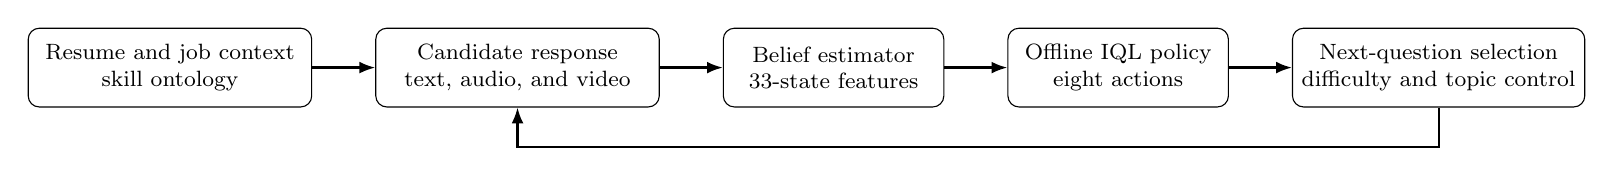
\begin{tikzpicture}[
node distance=6mm and 8mm,
block/.style={draw,rounded corners,align=center,minimum height=10mm,minimum width=28mm,font=\footnotesize},
wide/.style={draw,rounded corners,align=center,minimum height=10mm,minimum width=36mm,font=\footnotesize},
arrow/.style={-{Latex[length=2mm]},thick}
]
\node[wide] (context) {Resume and job context\\skill ontology};
\node[wide,right=of context] (response) {Candidate response\\text, audio, and video};
\node[block,right=of response] (belief) {Belief estimator\\33-state features};
\node[block,right=of belief] (policy) {Offline IQL policy\\eight actions};
\node[wide,right=of policy] (question) {Next-question selection\\difficulty and topic control};
\draw[arrow] (context) -- (response);
\draw[arrow] (response) -- (belief);
\draw[arrow] (belief) -- (policy);
\draw[arrow] (policy) -- (question);
\draw[arrow] (question.south) -- ++(0,-5mm) -| (response.south);
\end{tikzpicture}
\caption{ARIA architecture. Resume and job context define the skill space, response evidence updates a 33-dimensional belief state, and the offline IQL policy selects among eight interview actions. The evaluated policy is not yet executed by the current live interface.}
\label{fig:aria-evidence-boundary}
\end{figure*}

The architecture is described in layers, following the transparent system presentation used in IEEE Access comparators \cite{kim2023fairness}, \cite{putra2024magbert}, \cite{suen2019personality}. Design lessons from 2026 papers remain future protocol requirements. PolyInterview's faithfulness result motivates transcript-grounded feedback checks \cite{wen2026polyinterview}; Cheng's bias-propagation analysis motivates fairness gates at data, belief, action, and outcome stages \cite{cheng2026fairness}; Sakib \emph{et al.}'s findings motivate response editing, control, and transparent feedback options \cite{sakib2026expecting}; and AVI-Personality motivates trait-activated prompts and behaviorally anchored human labels \cite{zhang2026avipersonality}. These elements are not evaluated ARIA features.


\subsection{State, Belief, and Actions}

The state vector has 33 dimensions: skill beliefs, uncertainty and entropy, coverage, difficulty, recent evidence, modality availability, temporal features, and session context. Eight discrete actions encode increasing or decreasing difficulty, continuing or switching topic, probing foundations, asking behavioral or situational questions, and concluding. Bounds and dimensions are checked during trajectory reconstruction and inference. This explicit representation makes each policy input and permissible action inspectable.


Let $\mathbf{b}_t$ denote the belief over skill level at turn $t$, and let $\mathbf{o}_t$ denote the observed response evidence. The calibrated update is
\begin{equation}
\mathbf{b}_{t+1}=U(\mathbf{b}_t,\mathbf{o}_t;\mathbf{c}),
\label{eq:belief-update}
\end{equation}
where $\mathbf{c}$ contains the calibration parameters. The policy state is
\begin{equation}
\mathbf{s}_t=\phi(\mathbf{b}_t,\mathbf{u}_t,\mathbf{h}_t,\mathbf{m}_t),
\label{eq:state-construction}
\end{equation}
where $\mathbf{u}_t$ is uncertainty, $\mathbf{h}_t$ summarizes interview history, and $\mathbf{m}_t$ contains modality and context indicators. Calibration is evaluated independently of policy action quality, consistent with the distinction between predictive confidence and decision utility \cite{guo2017calibration}, \cite{malinin2017uncertainty}.


\section{Training Methodology}

\subsection{Synthetic Trajectories and Leakage Control}

The production corpus contains 600 episodes and 9,018 transitions. It is derived from 60 resume--job-description pairs expanded through paraphrase and perturbation variants. Leakage control operates on connected identity components rather than row identity. Thirty-three components are assigned wholly to train, validation, or test, producing 422/87/91 episodes and zero cross-split component overlap. Labels are balanced at 200 low, 200 medium, and 200 high episodes. All eight actions occur in the corpus.


Synthetic data permits controlled engineering tests but does not reproduce real applicant distributions, disability access needs, strategic behavior, or employment criteria. The 2026 disability studies \cite{luria2026disability}, \cite{kameswaran2026surveilling} and multidisciplinary reviews \cite{hunkenschroer2022ethics}, \cite{hughes2025inequalities}, \cite{zhao2026recruitingagents} make this limitation substantive: identity-safe splitting prevents one form of leakage, not population or construct invalidity. Table~\ref{tab:corpus-inventory} summarizes the corpus and split checks.


\begin{table}[htbp]
\caption{Synthetic Corpus Inventory}
\label{tab:corpus-inventory}
\centering
\small
\begin{tabularx}{\linewidth}{>{\raggedright\arraybackslash}X>{\raggedright\arraybackslash}X>{\raggedright\arraybackslash}X}
\toprule
Dataset property & Value & Evaluation check \\ \midrule
Episodes & 600 & Complete corpus count \\
Transitions & 9,018 & Complete transition count \\
Identity components & 33 & Connected-component analysis \\
Train / validation / locked test & 422 / 87 / 91 & Identity-isolated partitioning \\
Synthetic labels & 200 / 200 / 200 & Full label distribution \\
Action support & 8 of 8 & Full action distribution \\
Cross-split component overlap & 0 & Component-isolation check \\
\bottomrule
\end{tabularx}
\end{table}

\subsection{IQL Optimization}

The IQL policy uses discount 0.99, target-update coefficient 0.005, expectile 0.8, inverse-temperature parameter 3.0, learning rate 0.0001, seed 42, patience 10, and best epoch 4. The validation objective of 4.13864 is a training-selection statistic, not an estimate of interview benefit. IQL was selected because it limits explicit maximization over actions that lack support in the offline data \cite{kostrikov2021iql}.

\section{Experimental Setup}

\subsection{Belief Calibration and Locked Evaluation}

The locked evaluation contains 91 test episodes across six identity components. It assesses belief estimation only and does not evaluate the learned policy. Metrics include accuracy and micro-F1, macro-F1, balanced accuracy, per-class precision, recall, and F1, minimum recall, ordinal mean absolute error (MAE), expected calibration error (ECE), Brier score, coverage, abstention, and prediction concentration. The confusion matrix uses true classes as rows and predicted classes as columns.


\subsection{Offline Policy Diagnostic}

Policy evaluation depends on overlap with the behavior policy. The clipped weighted-importance-sampling diagnostic uses 1,405 validation transitions and a clip threshold of 20. It reports an estimate of 0.4618, effective sample size 1003.5, maximum importance ratio 5.464, and zero clipped ratios. In accordance with OPE guidance \cite{thomas2015hcope}--\cite{patterson2023empirical}, this diagnostic does not establish policy effectiveness. Fresh fixed-cycle, random-valid-action, uncertainty-greedy, and IQL rollouts are required.


\subsection{Verification Protocol}

Experimental verification combined state-schema checks, complete corpus validation, identity-overlap analysis, policy-parameter inspection, and focused regression tests. The focused belief and offline-policy suite produced 341 passing tests. These checks support consistency of the evaluated pipeline, but they do not substitute for human construct validation, subgroup evaluation, or end-to-end policy testing.


\section{Results and Analysis}

\subsection{Locked Belief Results}

The locked belief evaluation achieved accuracy and micro-F1 0.9121, macro-F1 0.9168, balanced accuracy 0.9227, minimum class recall 0.8286, ordinal MAE 0.0879, ECE 0.0870, and Brier score 0.1395. Coverage was 1.0 with no abstentions. Class recalls were 0.8286, 0.9394, and 1.0000 for low, medium, and high; corresponding F1 values were 0.9063, 0.8857, and 0.9583. Table~\ref{tab:belief-results} and Fig.~\ref{fig:belief-metric-comparison} compare these values with the preceding calibration model.


\begin{table}[htbp]
\caption{Paired Locked Belief Evaluation}
\label{tab:belief-results}
\centering
\small
\begin{tabularx}{\linewidth}{>{\raggedright\arraybackslash}X>{\raggedright\arraybackslash}X>{\raggedright\arraybackslash}X>{\raggedright\arraybackslash}X}
\toprule
Metric & Previous model & Calibrated model & Difference \\ \midrule
Accuracy / micro-F1 & 0.7912 & 0.9121 & +0.1209 \\
Macro-F1 & 0.8010 & 0.9168 & +0.1158 \\
Balanced accuracy & 0.8179 & 0.9227 & +0.1048 \\
Minimum class recall & 0.5143 & 0.8286 & +0.3143 \\
ECE & 0.0808 & 0.0870 & +0.0062 \\
Brier score & 0.2451 & 0.1395 & $-0.1055$ \\
Ordinal MAE & 0.2088 & 0.0879 & $-0.1209$ \\
\bottomrule
\end{tabularx}
\end{table}

\begin{figure}[htbp]
\centering
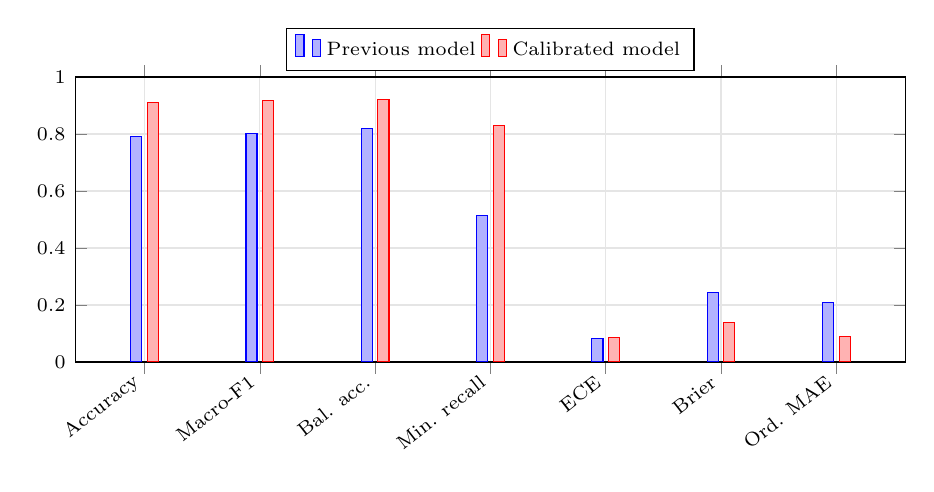
\begin{tikzpicture}
\begin{axis}[
width=\linewidth,height=5.2cm,
ybar,bar width=4pt,ymin=0,ymax=1,
symbolic x coords={Accuracy,Macro-F1,Bal. acc.,Min. recall,ECE,Brier,Ord. MAE},
xtick=data,x tick label style={rotate=38,anchor=east,font=\scriptsize},
yticklabel style={font=\scriptsize},
legend style={font=\scriptsize,at={(0.5,1.02)},anchor=south,legend columns=2},
grid=major,grid style={gray!20}
]
\addplot coordinates {(Accuracy,0.7912) (Macro-F1,0.8010) (Bal. acc.,0.8179) (Min. recall,0.5143) (ECE,0.0808) (Brier,0.2451) (Ord. MAE,0.2088)};
\addplot coordinates {(Accuracy,0.9121) (Macro-F1,0.9168) (Bal. acc.,0.9227) (Min. recall,0.8286) (ECE,0.0870) (Brier,0.1395) (Ord. MAE,0.0879)};
\legend{Previous model,Calibrated model}
\end{axis}
\end{tikzpicture}
\caption{Paired locked synthetic belief metrics. Higher is better for accuracy, macro-F1, balanced accuracy, and minimum recall; lower is better for ECE, Brier score, and ordinal MAE.}
\label{fig:belief-metric-comparison}
\end{figure}

The paired identity-component bootstrap reports a 95\% interval of 0.0435--0.2235 for the accuracy difference and 0.0443--0.1976 for the macro-F1 difference. The positive intervals support non-regression on this synthetic locked set. ECE increased by 0.0062, with a bootstrap interval spanning negative and positive values, whereas Brier score decreased. This mixed calibration result is why both reliability-sensitive and class-sensitive metrics are retained \cite{guo2017calibration}. Figure~\ref{fig:belief-confusion-matrix} shows that all eight errors are between adjacent skill levels.


\begin{figure}[htbp]
\centering
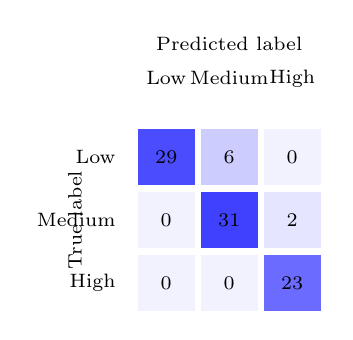
\begin{tikzpicture}[x=8mm,y=8mm,font=\scriptsize]
\foreach \x/\label in {0/Low,1/Medium,2/High}{\node at (\x,3.25) {\label};}
\foreach \y/\label in {2/Low,1/Medium,0/High}{\node[anchor=east] at (-0.65,\y) {\label};}
\foreach \x/\y/\value/\shade in {
0/2/29/70,1/2/6/20,2/2/0/5,
0/1/0/5,1/1/31/75,2/1/2/10,
0/0/0/5,1/0/0/5,2/0/23/58}{
\fill[blue!\shade] (\x-0.45,\y-0.45) rectangle (\x+0.45,\y+0.45);
\node at (\x,\y) {\value};}
\node at (1,3.8) {Predicted label};
\node[rotate=90] at (-1.45,1) {True label};
\end{tikzpicture}
\caption{Confusion matrix for the locked synthetic belief evaluation ($n=91$). Rows are true labels and columns are predicted labels; all eight errors are adjacent-class errors.}
\label{fig:belief-confusion-matrix}
\end{figure}

\subsection{Corpus and Policy Diagnostics}

The corpus passed the state-schema, distribution, and split-isolation checks. Each action has support, but support alone does not guarantee adequate state--action coverage. The WIS result is numerically stable under its clip threshold, as indicated by the effective sample size and absence of clipping. It remains a validation-set diagnostic because estimated propensities, synthetic rewards, and policy mismatch can bias the estimate \cite{thomas2015hcope}, \cite{voloshin2019ope}. No confidence-bound release rule was satisfied, so fresh rollout comparison remains necessary. Table~\ref{tab:policy-diagnostic} separates training evidence from claims that remain unsupported.


\begin{table}[htbp]
\caption{Offline Training and Policy Diagnostic Summary}
\label{tab:policy-diagnostic}
\centering
\small
\begin{tabularx}{\linewidth}{>{\raggedright\arraybackslash}X>{\raggedright\arraybackslash}X>{\raggedright\arraybackslash}X}
\toprule
Evidence item & Result & Correct interpretation \\ \midrule
Focused belief and policy tests & 341 passed & Consistency evidence for evaluated operations \\
Live interface integration & Incomplete & Learned policy is not executed end to end \\
IQL best epoch / validation objective & 4 / 4.13864 & Training trace, not deployment effect \\
Validation WIS estimate & 0.4618 & Diagnostic estimate only \\
WIS ESS / maximum ratio & 1003.5 / 5.464 & Numerically usable sample, not causal identification \\
Policy-release criterion & Not satisfied & Learned-policy effectiveness remains unverified \\
\bottomrule
\end{tabularx}
\end{table}

\subsection{Comparison With Existing Approaches}

ARIA's locked belief accuracy should not be ranked directly against published interview systems because labels, populations, tasks, and outcomes differ. Naim et al. \cite{naim2018automated}, HireNet \cite{hemamou2019hirenet}, and IEEE Access systems \cite{kim2023fairness}, \cite{putra2024magbert}, \cite{suen2019personality} predict human judgments or personality-related targets from real videos. PolyInterview evaluates question and feedback quality \cite{wen2026polyinterview}. AVI-Personality evaluates continuous traits and competencies with expert ratings \cite{zhang2026avipersonality}. ARIA evaluates synthetic categorical beliefs. A numerical leaderboard across these studies would be invalid.


The meaningful comparison is methodological. ARIA separates belief evaluation, off-policy diagnostics, and live execution. Conversely, ARIA is weaker in human evidence. It has no participant study comparable to PolyInterview's expert assessment \cite{wen2026polyinterview}, no psychometric label construction comparable to AVI-Personality \cite{zhang2026avipersonality}, no fairness experiment comparable to Kim \emph{et al.} or Putra \emph{et al.} \cite{kim2023fairness}, \cite{putra2024magbert}, and no accessibility study comparable to Luria \emph{et al.} or Kameswaran \emph{et al.} \cite{luria2026disability}, \cite{kameswaran2026surveilling}.


\subsection{Discussion}

The results support a calibrated synthetic belief component and a reproducible offline-learning procedure. They do not establish that adaptive questions improve interviews. Stored-state prediction and sequential policy value are different estimands. The improvement is meaningful within the paired locked evaluation, but the test contains only six identity components; component-level intervals should therefore be interpreted as diagnostic rather than population-general confidence intervals.


The 2026 literature also changes the model-development priorities. PolyInterview's low faithfulness rating for polished responses indicates that feedback must remain anchored to the candidate transcript \cite{wen2026polyinterview}. AVI-Personality suggests that future human data should use construct-targeted prompts and trained behaviorally anchored raters, followed by modality ablations \cite{zhang2026avipersonality}. Cheng's analysis requires fairness evaluation across administration, evidence extraction, belief update, action selection, and final feedback---not only output parity \cite{cheng2026fairness}. Sakib et al. show that user control and feedback design affect confidence, expressiveness, and perceived usefulness \cite{sakib2026expecting}. These findings justify four release prerequisites: grounded feedback checks, psychometric labeling, pipeline-wide subgroup audits, and candidate control mechanisms.


Accessibility is a decisive limitation. Disability-related communication patterns can be misread as low competence, and inaccessible interfaces can prevent completion before any model prediction occurs \cite{buyl2022disability}, \cite{benson2024autistic}, \cite{luria2026disability}--\cite{tilmes2022disability}, \cite{fisher2024disability}. The live system must therefore provide keyboard and screen-reader compatibility, alternatives to timed audiovisual response, accommodation controls, editing or re-recording without penalty, and human appeal. It should remain a practice and research tool, not an autonomous gatekeeper.


Privacy and contestability are similarly unresolved. Audio/video signals can reveal sensitive attributes, and emotion analysis may produce surveillance and self-presentation harms \cite{pyle2024justice}, \cite{aizenberg2023autonomy}, \cite{ingber2025emotion}, \cite{roemmich2023values}, \cite{liu2023uncertainty}, \cite{roemmich2023privacy}. Future work must minimize retention, separate raw media from derived features, document consent and deletion, disclose model limits, and permit human review. Auditability cannot be reduced to an internal log; outside access and institutional accountability matter \cite{kazim2021audit}, \cite{wilson2021fairalgorithms}, \cite{mihaljevic2023auditing}, \cite{gerchick2025audits}, \cite{costanzachock2022auditors}, \cite{raji2022oversight}.


\subsection{Threats to Validity and Non-Claims}

Construct validity is absent because labels are synthetic. External validity is absent because no real candidate population or job-performance criterion was evaluated. Policy validity is absent because there are no fresh learned-policy rollouts. Fairness validity is absent because demographic, disability, intersectional, and accessibility outcomes were not measured. Integration validity is limited because the live application does not run the evaluated offline stack. Statistical precision is limited by six locked-test identity components, even though the episode count is 91.


Accordingly, this paper does not claim that ARIA identifies competent candidates, improves hiring, is demographically fair, is accessible, outperforms human interviewers, or is production-ready. It also does not interpret contextual behavioral cues as verified competence. The reported validation applies only to the specified synthetic belief evaluation.


\section{Conclusion}

ARIA's defensible present contribution is an auditable offline architecture for studying adaptive mock interviews. The system connects a 33-dimensional state, eight actions, an identity-isolated 600-episode synthetic corpus, a calibrated 91-episode locked belief evaluation, and a trained IQL policy with a conservative diagnostic OPE result. The strongest result is the calibrated belief performance of 0.9121 accuracy, 0.9168 macro-F1, and 0.0870 ECE, together with explicit evidence that these numbers do not evaluate the learned policy.


The next study should execute fresh held-out rollouts against fixed-cycle, random-valid-action, and uncertainty-greedy baselines; report component-level uncertainty; and keep the locked test isolated. A separately governed human study should use construct-targeted questions, trained behaviorally anchored raters, accessible interaction alternatives, modality ablations, subgroup calibration and error analysis, candidate-reaction measures, and human appeal. Until those studies are completed, ARIA should be presented as a transparent research prototype for mock-interview experimentation, not a hiring decision system.


\begin{thebibliography}{99}
\bibitem{hemamou2019hirenet} L. Hemamou, G. Felhi, V. Vandenbussche, J.-C. Martin, and C. Clavel, ``HireNet: A Hierarchical Attention Model for the Automatic Analysis of Asynchronous Video Job Interviews,'' in \emph{Proceedings of the AAAI Conference on Artificial Intelligence}, 2019. doi: \href{https://doi.org/10.1609/aaai.v33i01.3301573}{10.1609/aaai.v33i01.3301573}.
\bibitem{naim2018automated} I. Naim, M. I. Tanveer, D. Gildea, and M. E. Hoque, ``Automated Analysis and Prediction of Job Interview Performance,'' \emph{IEEE Transactions on Affective Computing}, 2018. doi: \href{https://doi.org/10.1109/TAFFC.2016.2614299}{10.1109/TAFFC.2016.2614299}.
\bibitem{hemamou2023multimodal} L. Hemamou, A. Guillon, J.-C. Martin, and C. Clavel, ``Multimodal Hierarchical Attention Neural Network: Looking for Candidates Behaviour Which Impact Recruiter's Decision,'' \emph{Ieee Transactions on Affective Computing}, 2023. doi: \href{https://doi.org/10.1109/taffc.2021.3113159}{10.1109/taffc.2021.3113159}.
\bibitem{nguyen2014hireme} L. S. Nguyen, D. Frauendorfer, M. S. Mast, and D. Gatica-Perez, ``Hire Me: Computational Inference of Hirability in Employment Interviews Based on Nonverbal Behavior,'' \emph{Ieee Transactions on Multimedia}, 2014. doi: \href{https://doi.org/10.1109/tmm.2014.2307169}{10.1109/tmm.2014.2307169}.
\bibitem{chen2016monologue} L. Chen et al., ``Automatic Scoring of Monologue Video Interviews Using Multimodal Cues,'' in \emph{Proceedings of Interspeech 2016}, 2016. doi: \href{https://doi.org/10.21437/interspeech.2016-1453}{10.21437/interspeech.2016-1453}.
\bibitem{lv2024window} J. Lv, C. Chen, and Z. Liang, ``Automated Scoring of Asynchronous Interview Videos Based on Multi-Modal Window-Consistency Fusion,'' \emph{Ieee Transactions on Affective Computing}, 2024. doi: \href{https://doi.org/10.1109/taffc.2023.3294335}{10.1109/taffc.2023.3294335}.
\bibitem{suen2020agent} H.-Y. Suen, K.-E. Hung, and C.-L. Lin, ``Intelligent Video Interview Agent Used to Predict Communication Skill and Perceived Personality Traits,'' \emph{Human-Centric Computing and Information Sciences}, 2020. doi: \href{https://doi.org/10.1186/s13673-020-0208-3}{10.1186/s13673-020-0208-3}.
\bibitem{chen2016doc2vec} L. Chen et al., ``Automated Scoring of Interview Videos Using Doc2Vec Multimodal Feature Extraction Paradigm,'' in \emph{Proceedings of the 18th ACM International Conference on Multimodal Interaction}, 2016. doi: \href{https://doi.org/10.1145/2993148.2993203}{10.1145/2993148.2993203}.
\bibitem{hickman2022personality} L. Hickman, N. Bosch, V. Ng, R. Saef, L. Tay, and S. E. Woo, ``Automated Video Interview Personality Assessments: Reliability, Validity, and Generalizability Investigations,'' \emph{Journal of Applied Psychology}, 2022. doi: \href{https://doi.org/10.1037/apl0000695}{10.1037/apl0000695}.
\bibitem{liff2024psychometric} J. Liff, N. Mondragon, C. Gardner, C. J. Hartwell, and A. L. Bradshaw, ``Psychometric Properties of Automated Video Interview Competency Assessments,'' \emph{Journal of Applied Psychology}, 2024. doi: \href{https://doi.org/10.1037/apl0001173}{10.1037/apl0001173}.
\bibitem{hickman2025smart} L. Hickman, L. Tay, and S. E. Woo, ``Are Automated Video Interviews Smart Enough? Behavioral Modes, Reliability, Validity, and Bias of Machine Learning Cognitive Ability Assessments.,'' \emph{Journal of Applied Psychology}, 2025. doi: \href{https://doi.org/10.1037/apl0001236}{10.1037/apl0001236}.
\bibitem{koutsoumpis2024psychometric} A. Koutsoumpis et al., ``Beyond Traditional Interviews: Psychometric Analysis of Asynchronous Video Interviews for Personality and Interview Performance Evaluation Using Machine Learning,'' \emph{Computers in Human Behavior}, 2024. doi: \href{https://doi.org/10.1016/j.chb.2023.108128}{10.1016/j.chb.2023.108128}.
\bibitem{hickman2024training} L. Hickman, J. Liff, C. Rottman, and C. Calderwood, ``The Effects of the Training Sample Size, Ground Truth Reliability, and NLP Method on Language-Based Automatic Interview Scores' Psychometric Properties,'' \emph{Organizational Research Methods}, 2024. doi: \href{https://doi.org/10.1177/10944281241264027}{10.1177/10944281241264027}.
\bibitem{hickman2021language} L. Hickman, R. Saef, V. Ng, S. E. Woo, L. Tay, and N. Bosch, ``Developing and Evaluating Language-based Machine Learning Algorithms for Inferring Applicant Personality in Video Interviews,'' \emph{Human Resource Management Journal}, 2021. doi: \href{https://doi.org/10.1111/1748-8583.12356}{10.1111/1748-8583.12356}.
\bibitem{zhang2025personality} T. Zhang et al., ``Assessing Personality Traits and Interview Performance From Asynchronous Video Interviews,'' in \emph{Proceedings of the 33rd ACM International Conference on Multimedia}, 2025. doi: \href{https://doi.org/10.1145/3746027.3762016}{10.1145/3746027.3762016}.
\bibitem{li2026deepcat} J. Li, R. Gibbons, and V. Rockova, ``Deep Computerized Adaptive Testing,'' \emph{arXiv preprint arXiv:2502.19275}, 2026. [Online]. Available: \url{https://arxiv.org/abs/2502.19275}.
\bibitem{kostrikov2021iql} I. Kostrikov, A. Nair, and S. Levine, ``Offline Reinforcement Learning with Implicit Q-Learning,'' \emph{arXiv preprint arXiv:2110.06169}, 2021. doi: \href{https://doi.org/10.48550/arXiv.2110.06169}{10.48550/arXiv.2110.06169}.
\bibitem{thomas2015hcope} P. S. Thomas, G. Theocharous, and M. Ghavamzadeh, ``High-Confidence Off-Policy Evaluation,'' in \emph{Proceedings of the AAAI Conference on Artificial Intelligence}, 2015. doi: \href{https://doi.org/10.1609/aaai.v29i1.9541}{10.1609/aaai.v29i1.9541}.
\bibitem{patterson2023empirical} A. D. Patterson, S. Neumann, M. White, and A. White, ``Empirical Design in Reinforcement Learning,'' \emph{arXiv preprint arXiv:2304.01315}, 2023. doi: \href{https://doi.org/10.48550/arXiv.2304.01315}{10.48550/arXiv.2304.01315}.
\bibitem{raghavan2020bias} M. Raghavan, S. Barocas, J. Kleinberg, and K. Levy, ``Mitigating Bias in Algorithmic Hiring: Evaluating Claims and Practices,'' in \emph{Proceedings of the 2020 Conference on Fairness, Accountability, and Transparency}, 2020. doi: \href{https://doi.org/10.1145/3351095.3372828}{10.1145/3351095.3372828}.
\bibitem{tippins2021concerns} N. T. Tippins, F. L. Oswald, and S. McPhail, ``Scientific, Legal, and Ethical Concerns About AI-Based Personnel Selection Tools: A Call to Action,'' \emph{Personnel Assessment and Decisions}, 2021. doi: \href{https://doi.org/10.31234/osf.io/6gczw}{10.31234/osf.io/6gczw}.
\bibitem{rhea2022stability} A. K. Rhea et al., ``An External Stability Audit Framework to Test the Validity of Personality Prediction in AI Hiring,'' \emph{Data Mining and Knowledge Discovery}, 2022. doi: \href{https://doi.org/10.1007/s10618-022-00861-0}{10.1007/s10618-022-00861-0}.
\bibitem{fabris2025survey} A. Fabris et al., ``Fairness and Bias in Algorithmic Hiring: A Multidisciplinary Survey,'' \emph{ACM Transactions on Intelligent Systems and Technology}, 2025. doi: \href{https://doi.org/10.1145/3696457}{10.1145/3696457}.
\bibitem{luria2026disability} M. Luria, A. Aboulafia, and D. Thakur, ``Disqualified by Disability: The Exclusion of Disabled Workers by Digitized Hiring Assessments,'' in \emph{Proceedings of the 2026 CHI Conference on Human Factors in Computing Systems}, 2026. doi: \href{https://doi.org/10.1145/3772318.3791485}{10.1145/3772318.3791485}.
\bibitem{wilson2021fairalgorithms} C. Wilson et al., ``Building and Auditing Fair Algorithms,'' in \emph{Proceedings of the 2021 ACM Conference on Fairness, Accountability, and Transparency}, 2021. doi: \href{https://doi.org/10.1145/3442188.3445928}{10.1145/3442188.3445928}.
\bibitem{hunkenschroer2022ethics} A. L. Hunkenschroer and C. Luetge, ``Ethics of AI-Enabled Recruiting and Selection: A Review and Research Agenda,'' \emph{Journal of Business Ethics}, 2022. doi: \href{https://doi.org/10.1007/s10551-022-05049-6}{10.1007/s10551-022-05049-6}.
\bibitem{aizenberg2023autonomy} E. Aizenberg, M. Dennis, and J. van den Hoven, ``Examining the Assumptions of AI Hiring Assessments and Their Impact on Job Seekers' Autonomy Over Self-Representation,'' \emph{Ai \& Society}, 2023. doi: \href{https://doi.org/10.1007/s00146-023-01783-1}{10.1007/s00146-023-01783-1}.
\bibitem{ingber2025emotion} A. S. Ingber and N. Andalibi, ``Emotion AI in Job Interviews: Injustice, Emotional Labor, Identity, and Privacy,'' in \emph{Proceedings of the 2025 ACM Conference on Fairness, Accountability, and Transparency}, 2025. doi: \href{https://doi.org/10.1145/3715275.3732002}{10.1145/3715275.3732002}.
\bibitem{roemmich2023values} K. Roemmich, T. I. Rosenberg, S. Fan, and N. Andalibi, ``Values in Emotion Artificial Intelligence Hiring Services: Technosolutions to Organizational Problems,'' \emph{Proceedings of the Acm on Human-Computer Interaction}, 2023. doi: \href{https://doi.org/10.1145/3579543}{10.1145/3579543}.
\bibitem{kassir2022context} S. Kassir, L. Baker, J. Dolphin, and F. Polli, ``AI for Hiring in Context: A Perspective on Overcoming the Unique Challenges of Employment Research to Mitigate Disparate Impact,'' \emph{Ai and Ethics}, 2022. doi: \href{https://doi.org/10.1007/s43681-022-00208-x}{10.1007/s43681-022-00208-x}.
\bibitem{li2021practice} L. Li, T. Lassiter, J. Oh, and M. K. Lee, ``Algorithmic Hiring in Practice,'' in \emph{Proceedings of the 2021 AAAI/ACM Conference on AI, Ethics, and Society}, 2021. doi: \href{https://doi.org/10.1145/3461702.3462531}{10.1145/3461702.3462531}.
\bibitem{gerchick2025audits} M. Gerchick, R. Encarnacion, C. Tanigawa-Lau, L. Armstrong, A. B. Gutierrez, and D. Metaxa, ``Auditing the Audits: Lessons for Algorithmic Accountability From Local Law 144's Bias Audits,'' in \emph{Proceedings of the 2025 ACM Conference on Fairness, Accountability, and Transparency}, 2025. doi: \href{https://doi.org/10.1145/3715275.3732004}{10.1145/3715275.3732004}.
\bibitem{fisher2024disability} S. L. Fisher, S. Bonaccio, and C. E. Connelly, ``AI-based Tools in Selection: Considering the Impact on Applicants With Disabilities,'' \emph{Organizational Dynamics}, 2024. doi: \href{https://doi.org/10.1016/j.orgdyn.2024.101036}{10.1016/j.orgdyn.2024.101036}.
\bibitem{yam2021impact} J. Yam and J. A. Skorburg, ``From Human Resources to Human Rights: Impact Assessments for Hiring Algorithms,'' \emph{Ethics and Information Technology}, 2021. doi: \href{https://doi.org/10.1007/s10676-021-09599-7}{10.1007/s10676-021-09599-7}.
\bibitem{roemmich2023privacy} K. Roemmich, F. Schaub, and N. Andalibi, ``Emotion AI at Work: Implications for Workplace Surveillance, Emotional Labor, and Emotional Privacy,'' in \emph{Proceedings of the 2023 CHI Conference on Human Factors in Computing Systems}, 2023. doi: \href{https://doi.org/10.1145/3544548.3580950}{10.1145/3544548.3580950}.
\bibitem{raji2022oversight} I. D. Raji, P. Xu, C. Honigsberg, and D. E. Ho, ``Outsider Oversight: Designing a Third Party Audit Ecosystem for AI Governance,'' in \emph{Proceedings of the 2022 AAAI/ACM Conference on AI, Ethics, and Society}, 2022. doi: \href{https://doi.org/10.1145/3514094.3534181}{10.1145/3514094.3534181}.
\bibitem{wen2026polyinterview} Z. Wen et al., ``PolyInterview: An LLM-based Platform for Immersive Mock Interview Practice with Comprehensive Multimodal Assessment,'' \emph{arXiv preprint arXiv:2607.10310}, 2026. [Online]. Available: \url{https://arxiv.org/abs/2607.10310}.
\bibitem{kameswaran2026surveilling} V. Kameswaran, V. Hong, J. Clark, Y. Hou, H. Daume III, and K. Shilton, ``Surveilling Suitability: How AI Hiring Interviews Impact Job Seekers With Disabilities,'' in \emph{Proceedings of the 2026 CHI Conference on Human Factors in Computing Systems}, 2026. doi: \href{https://doi.org/10.1145/3772318.3791516}{10.1145/3772318.3791516}.
\bibitem{cheng2026fairness} Y. Cheng, ``Fairness Issues and Evaluation in Psychometrics and AI/ML: What Can We Learn From Each Field?,'' \emph{Psychometrika}, 2026. doi: \href{https://doi.org/10.1017/psy.2026.10110}{10.1017/psy.2026.10110}.
\bibitem{zhao2026recruitingagents} Z. Zhao and G. Wei, ``From Matching Models to Recruiting Agents: A Systematized Narrative Review of AI Recruitment Systems, Evaluation, and Governance,'' \emph{arXiv preprint arXiv:2609.04286}, 2026. [Online]. Available: \url{https://arxiv.org/abs/2609.04286}.
\bibitem{sakib2026expecting} M. N. Sakib, N. M. Rayasam, and S. Dey, ``Expecting Too Much, Getting Too Little: Exploring the Challenges and Design Opportunities of Asynchronous AI Interviewers,'' \emph{arXiv preprint arXiv:2601.02775}, 2026. [Online]. Available: \url{https://arxiv.org/abs/2601.02775}.
\bibitem{zhang2026avipersonality} T. Zhang, J. Shang, A. Koutsoumpis, Y. Zong, R. E. de Vries, and W. Zheng, ``AVI-Personality: A Trait-Activated Multimodal Dataset for Personality and Competency Assessment in Asynchronous Video Interviews,'' \emph{arXiv preprint arXiv:2608.25316}, 2026. [Online]. Available: \url{https://arxiv.org/abs/2608.25316}.
\bibitem{kim2023fairness} C. Kim, J.-H. Choi, J. Yoon, D. Yoo, and W. Lee, ``Fairness-Aware Multimodal Learning in Automatic Video Interview Assessment,'' \emph{Ieee Access}, 2023. doi: \href{https://doi.org/10.1109/access.2023.3325891}{10.1109/access.2023.3325891}.
\bibitem{putra2024magbert} B. Putra et al., ``MAG-BERT-ARL for Fair Automated Video Interview Assessment,'' \emph{Ieee Access}, 2024. doi: \href{https://doi.org/10.1109/access.2024.3473314}{10.1109/access.2024.3473314}.
\bibitem{suen2019personality} H.-Y. Suen, K.-E. Hung, and C.-L. Lin, ``TensorFlow-Based Automatic Personality Recognition Used in Asynchronous Video Interviews,'' \emph{Ieee Access}, 2019. doi: \href{https://doi.org/10.1109/access.2019.2902863}{10.1109/access.2019.2902863}.
\bibitem{levashina2014structured} J. Levashina, C. J. Hartwell, F. P. Morgeson, and M. A. Campion, ``The Structured Employment Interview: Narrative and Quantitative Review of the Research Literature,'' \emph{Personnel Psychology}, 2014. doi: \href{https://doi.org/10.1111/peps.12052}{10.1111/peps.12052}.
\bibitem{mcdaniel1994validity} M. A. McDaniel, D. L. Whetzel, F. L. Schmidt, and S. D. Maurer, ``The Validity of Employment Interviews: A Comprehensive Review and Meta-Analysis.,'' \emph{Journal of Applied Psychology}, 1994. doi: \href{https://doi.org/10.1037/0021-9010.79.4.599}{10.1037/0021-9010.79.4.599}.
\bibitem{hickman2025asr} L. Hickman, M. Langer, R. Saef, and L. Tay, ``Automated Speech Recognition Bias in Personnel Selection: The Case of Automatically Scored Job Interviews,'' \emph{Journal of Applied Psychology}, 2025. doi: \href{https://doi.org/10.1037/apl0001247}{10.1037/apl0001247}.
\bibitem{hickman2025faking} L. Hickman, J. Liff, C. Willis, and E. H. Kim, ``Can Interviewees Fake Out AI? Comparing the Susceptibility and Mechanisms of Faking Across Self-Reports, Human Interview Ratings, and AI Interview Ratings,'' \emph{International Journal of Selection and Assessment}, 2025. doi: \href{https://doi.org/10.1111/ijsa.70014}{10.1111/ijsa.70014}.
\bibitem{booth2021bias} B. M. Booth, L. Hickman, S. K. Subburaj, L. Tay, S. E. Woo, and S. K. D'Mello, ``Bias and Fairness in Multimodal Machine Learning: A Case Study of Automated Video Interviews,'' in \emph{Proceedings of the 2021 International Conference on Multimodal Interaction}, 2021. doi: \href{https://doi.org/10.1145/3462244.3479897}{10.1145/3462244.3479897}.
\bibitem{malinin2017uncertainty} A. Malinin, A. Ragni, K. Knill, and M. Gales, ``Incorporating Uncertainty Into Deep Learning for Spoken Language Assessment,'' in \emph{Proceedings of the 55th Annual Meeting of the Association for Computational Linguistics: Student Research Workshop}, 2017. doi: \href{https://doi.org/10.18653/v1/p17-2008}{10.18653/v1/p17-2008}.
\bibitem{qin2023question} C. Qin et al., ``Automatic Skill-Oriented Question Generation and Recommendation for Intelligent Job Interviews,'' \emph{Acm Transactions on Information Systems}, 2023. doi: \href{https://doi.org/10.1145/3604552}{10.1145/3604552}.
\bibitem{segall2025items} D. Segall and T. Kantrowitz, ``Harnessing Generative AI for Assessment Item Development: Comparing AI-Generated and Human-Authored Items,'' \emph{International Journal of Selection and Assessment}, 2025. doi: \href{https://doi.org/10.1111/ijsa.70021}{10.1111/ijsa.70021}.
\bibitem{voloshin2019ope} C. Voloshin, H. Le, N. Jiang, and Y. Yue, ``Empirical Study of Off-Policy Policy Evaluation for Reinforcement Learning,'' \emph{arXiv preprint arXiv:1911.06854}, 2019. doi: \href{https://doi.org/10.48550/arXiv.1911.06854}{10.48550/arXiv.1911.06854}.
\bibitem{hughes2025inequalities} K. D. Hughes, A. Konnikov, N. Denier, and Y. Hu, ``Problematizing the Role of Artificial Intelligence in Hiring and Organizational Inequalities: A Multidisciplinary Review,'' \emph{Human Relations}, 2025. doi: \href{https://doi.org/10.1177/00187267251403902}{10.1177/00187267251403902}.
\bibitem{kazim2021audit} E. Kazim, A. Koshiyama, A. Hilliard, and R. Polle, ``Systematizing Audit in Algorithmic Recruitment,'' \emph{Journal of Intelligence}, 2021. doi: \href{https://doi.org/10.3390/jintelligence9030046}{10.3390/jintelligence9030046}.
\bibitem{mihaljevic2023auditing} H. Mihaljevic, I. Muller, K. Dill, A. Yollu-Tok, and M. von Grafenstein, ``More or Less Discrimination? Practical Feasibility of Fairness Auditing of Technologies for Personnel Selection,'' \emph{Ai \& Society}, 2023. doi: \href{https://doi.org/10.1007/s00146-023-01726-w}{10.1007/s00146-023-01726-w}.
\bibitem{costanzachock2022auditors} S. Costanza-Chock, I. D. Raji, and J. Buolamwini, ``Who Audits the Auditors? Recommendations From a Field Scan of the Algorithmic Auditing Ecosystem,'' in \emph{Proceedings of the 2022 ACM Conference on Fairness, Accountability, and Transparency}, 2022. doi: \href{https://doi.org/10.1145/3531146.3533213}{10.1145/3531146.3533213}.
\bibitem{acikgoz2020justice} Y. Acikgoz, H. K. Davison, M. Compagnone, and M. M. Laske, ``Justice Perceptions of Artificial Intelligence in Selection,'' \emph{International Journal of Selection and Assessment}, 2020. doi: \href{https://doi.org/10.1111/ijsa.12306}{10.1111/ijsa.12306}.
\bibitem{oostrom2023reactions} J. K. Oostrom, D. Holtrop, A. Koutsoumpis, W. van Breda, S. Ghassemi, and R. E. de Vries, ``Applicant Reactions to Algorithm- versus Recruiter-based Evaluations of an Asynchronous Video Interview and a Personality Inventory,'' \emph{Journal of Occupational and Organizational Psychology}, 2023. doi: \href{https://doi.org/10.1111/joop.12465}{10.1111/joop.12465}.
\bibitem{pyle2024justice} C. Pyle, K. Roemmich, and N. Andalibi, ``U.S. Job-Seekers' Organizational Justice Perceptions of Emotion AI-Enabled Interviews,'' \emph{Proceedings of the ACM on Human-Computer Interaction}, 2024. doi: \href{https://doi.org/10.1145/3686993}{10.1145/3686993}.
\bibitem{langer2019acceptance} M. Langer, C. J. Konig, and M. Papathanasiou, ``Highly automated Job Interviews: Acceptance Under the Influence of Stakes,'' \emph{International Journal of Selection and Assessment}, 2019. doi: \href{https://doi.org/10.1111/ijsa.12246}{10.1111/ijsa.12246}.
\bibitem{liu2023uncertainty} B. Liu, L. Wei, M. Wu, and T. Luo, ``Speech Production Under Uncertainty: How Do Job Applicants Experience and Communicate With an AI Interviewer?,'' \emph{Journal of Computer-Mediated Communication}, 2023. doi: \href{https://doi.org/10.1093/jcmc/zmad028}{10.1093/jcmc/zmad028}.
\bibitem{hilliard2022perceived} A. Hilliard, N. Guenole, and F. Leutner, ``Robots Are Judging Me: Perceived Fairness of Algorithmic Recruitment Tools,'' \emph{Frontiers in Psychology}, 2022. doi: \href{https://doi.org/10.3389/fpsyg.2022.940456}{10.3389/fpsyg.2022.940456}.
\bibitem{sanchezmonedero2020discrimination} J. Sanchez-Monedero, L. Dencik, and L. Edwards, ``What Does It Mean to 'Solve' the Problem of Discrimination in Hiring?,'' in \emph{Proceedings of the 2020 Conference on Fairness, Accountability, and Transparency}, 2020. doi: \href{https://doi.org/10.1145/3351095.3372849}{10.1145/3351095.3372849}.
\bibitem{sloane2022auditability} M. Sloane, E. Moss, and R. Chowdhury, ``A Silicon Valley Love Triangle: Hiring Algorithms, Pseudo-Science, and the Quest for Auditability,'' \emph{Patterns}, 2022. doi: \href{https://doi.org/10.1016/j.patter.2021.100425}{10.1016/j.patter.2021.100425}.
\bibitem{buyl2022disability} M. Buyl, C. Cociancig, C. Frattone, and N. Roekens, ``Tackling Algorithmic Disability Discrimination in the Hiring Process,'' in \emph{Proceedings of the 2022 ACM Conference on Fairness, Accountability, and Transparency}, 2022. doi: \href{https://doi.org/10.1145/3531146.3533169}{10.1145/3531146.3533169}.
\bibitem{tilmes2022disability} N. Tilmes, ``Disability, Fairness, and Algorithmic Bias in AI Recruitment,'' \emph{Ethics and Information Technology}, 2022. doi: \href{https://doi.org/10.1007/s10676-022-09633-2}{10.1007/s10676-022-09633-2}.
\bibitem{benson2024autistic} A. L. Benson, K. L. Colley, J. J. Prasad, C. Willis, and T. Powell-Rudy, ``Comparing Autistic and Neurotypical Responses to Conventional and Modified Questions in Algorithmically Scored Asynchronous Video Interviews,'' \emph{International Journal of Selection and Assessment}, 2024. doi: \href{https://doi.org/10.1111/ijsa.12512}{10.1111/ijsa.12512}.
\bibitem{guo2017calibration} C. Guo, G. Pleiss, Y. Sun, and K. Q. Weinberger, ``On Calibration of Modern Neural Networks,'' \emph{Proceedings of Machine Learning Research}, 2017. [Online]. Available: \url{https://proceedings.mlr.press/v70/guo17a.html}.
\end{thebibliography}
\end{document}
